
\documentclass[11pt]{article}

\usepackage{common}
\title{HW4: Word Segmentation}
\author{Virgile Audi \\ vaudi@g.harvard.edu \\ Nicolas Drizard \\ nicolasdrizard@g.harvard.edu}
\begin{document}

\maketitle{}
\section{Introduction}

The goal of this assignement is to implement reccurent neural networks for a word segmentation task. The idea is to identify the spaces in sentence based on the previous characters only. This could be particularly helpful for processing languages written without spaces such as Korean or Spanish


\section{Problem Description}

The problem that needs to be solve in this homework is the following: given a sequence of characters, predict where to insert spaces to make a valid sentence. For instance, consider the following sequence of character:
\begin{center}
I A M A STUDENT IN C S 2 8 7\\
\end{center}
the implemented algorithm should be capable of segmenting this sequence into valid words to give:
\begin{center}
I am a student in CS 287\\
\end{center}

\noindent To solve this problem, we will train different language models including count-based models, basic neural networks, and recurrent neural networks, combined with two search algorithms to predict the right position for spaces, i.e. a greedy search algorithm and the Viturbi algorithm. 


\section{Model and Algorithms}

\subsection{Count-based Model}

The first model is a count-based character n-gram model. The goal is to compute the probability of the newt word being a space:

\[ P(w_i =<\mathrm{space}> | w_{i-n+1}, \ldots w_{i-1}) \]

This model is built by computing its MLE which gives:

\[ P(w_i =<\mathrm{space}> | w_{i-n+1}, \ldots w_{i-1}) = \frac{F_{c_i,s}}{F_{c_i,.}}\]

where $c_i = w_{i-n+1}, \ldots w_{i-1}$ is the context for the word $w_i$. We add a smoothing parameter $\alpha = 0.1$ just for the rare corner cases where the context was unseen (which is really rare in comparison to count-based word level models).

\subsection{Neural Language Model}
As a second baseline, we implemented a neural language model to predict whether the next character is a space or not. The model is similar to the Bengio model coded in HW3 but is adapted to characters. Similarly to what we did for word prediction, we imbed a window of characters in a higher dimension using a look-up table. We first apply a first linear model to the higher dimensional representation of the window of characters, followed by a hyperbolic tangent layer to extract non-linear features. A second linear layer is then applied followed by a softmax to get a probability distribution over the two possible outputs, i.e. a character or a space.\\
\noindent We can summarize the model in the following formula: $$nnlm_1(x) = \tanh(\mathbf{xW}+\mathbf{b})\mathbf{W'}+\mathbf{b'}$$
where we recall:
\begin{itemize}
\item $\boldsymbol{x}\in \Re^{d_{in}\cdot d_{win}}$ is the concatenated character embeddings
\item $\boldsymbol{W}\in \Re^{(d_{in}\cdot d_{win})\times d_{hid}}$, and $\boldsymbol{b}\in \Re^{d_{hid}}$
\item $\boldsymbol{W'}\in \Re^{d_{hid}\times 2}$, and $\boldsymbol{b'}\in \Re^{2}$.
\end{itemize}


\subsection{Algorithm to generate spaces sequences}
As mentioned in the problem description, in order to predict the position of a space, we will use two search algorithm. Both of these algorithm use the language models mentioned above to predict the next character or space given the prior context.

\subsubsection{Greedy}
The greedy algorithm implemented is an algorithm that chooses the locally optimum choice at every step in the sequence. This algorithm does not generally lead to a global maxium but has the advantage of being easilly implementable and efficient both in memory and complexity. The pseudo-code of the algorithm is presented below:

 \begin{algorithmic}[1]
    \Procedure{GreedySearch}{}
    \State{s=0}
    \State{$c\in \mathcal{C}^{n+1}$}
    \State{$c_0 = \langle s \rangle$}
    \For{i = 1 to n}
    \State{Predict the distribution $\mathbf{\hat{y}}$ over the two classes given the previous context}
    \State{Pick the next class that maximises the distribution $c_i \leftarrow \arg\max\limits_{c'_i}\mathbf{\hat{y}}(c_{i-1})_{c_i}$}
    \State{Update the score of the chain: $s+\log\mathbf{\hat{y}(c_{i-1})}_{c_i}$}
    \State{Update the chain/context by adding a space or the following character}
    \EndFor{}
	\Return{the chain and the score}
    \EndProcedure{}
  \end{algorithmic}
\subsubsection{Viterbi}
The second search algorithm that we implemented is the dynamic programming algorithm named after Andrew Viterbi. The main difference between t

\subsection{Recurrent Neural Networks}

We implemented three different recurrent neural networks and benchmark their performance in our experiments. The main point is that we want to compute one output for each timestep and not only for the last one, that's why the generic structure of our networks is a tranducer.

\paragraph{Generic RNN Transducer}

The motivation is to maintain history in the model by the introduction of hidden states at each time steps (here each character of the input sequence). The model contains two main transformation: the transition function that define the hidden state given $\mathbb{s_{i}}$ the current input $x_i$ and the previous hidden state $\mathbb{s_{i-1}}$ and the output layer producing the output $\mathbb{y_i}$ at each timestep. We used Elman tanh layer for the output.

\begin{figure}[H]
\begin{center}
    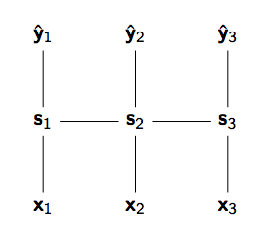
\includegraphics[width=0.45\textwidth]{transducer.png}
    \caption{Transducer Architecture}
\end{center}
\end{figure}

Formally:

\begin{align*}
\mathbb{\hat{y_i}} = softmax(\mathbb{s_i} \mathbb{W} + \mathbb{b}) \\
\mathbb{s_i} = tanh( [\mathbb{x_i}, \mathbb{s_{i-1}}\mathbb{W} + \mathbb{b})
\end{align*}

We used a batch version to learn the model and split the batched sequences in small chunks of characters of a given length to do the backpropagation to make it run faster. We explored different values for the two parameters length and batch size. 


\paragraph{GRU}

This models introduces the gating operation that allows a vector $\mathbb{t}$ to mask or gate $\mathbb{x}$. This operation is smoothed with a sigmoid: $t = \sigma(\mathbb{W^t}\mathbb{x} + \mathbb{b})$. This operation is used to stop connection by applying the reset gate $\mathbb{r}$. This operation may be useful to avoid issue with the long sequence of gradients we need to compute in the backpropagation phase.

Formally:

\begin{figure}[H]
\begin{center}
    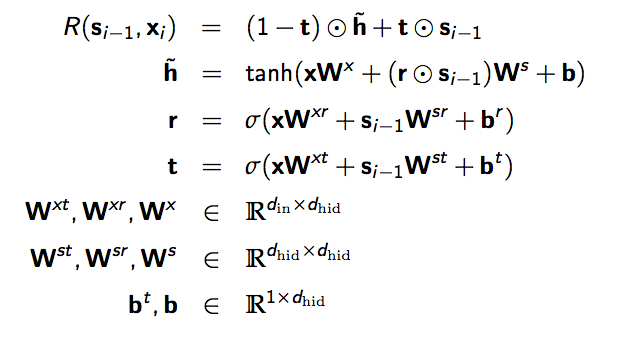
\includegraphics[width=0.45\textwidth]{gru.png}
    \caption{GRU equations}
\end{center}
\end{figure}

\paragraph{LSTM}

The long short term memory network uses also the gate idea with three gates: input, output and forget.

\begin{figure}[H]
\begin{center}
    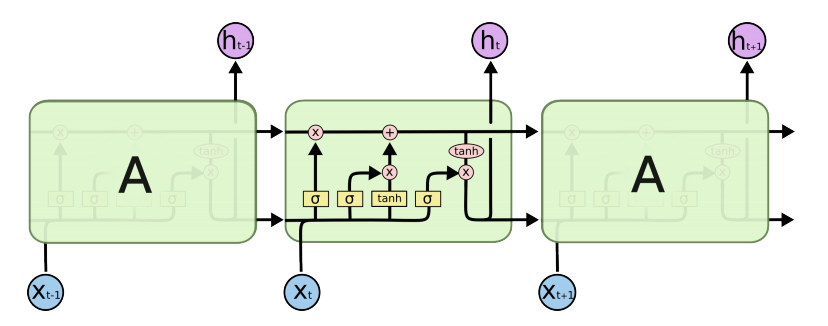
\includegraphics[width=0.45\textwidth]{lstm.png}
    \caption{LSTM Architecture}
\end{center}
\end{figure}

Formally:

\begin{figure}[H]
\begin{center}
    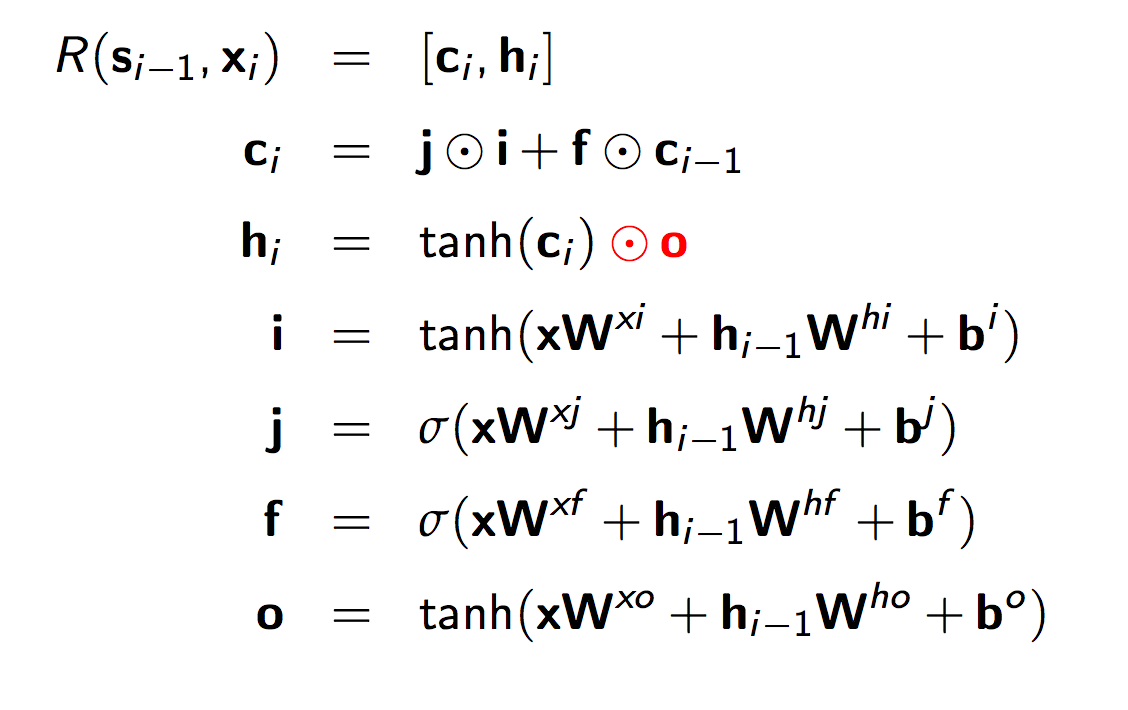
\includegraphics[width=0.45\textwidth]{lstm_eq.png}
    \caption{Perplexity evolution for the GRU}
\end{center}
\end{figure}


\section{Experiments}

\subsection{Count-based Model}

This first approach relies on a window approach where we predict the next character given a fixed size of previous character. This size is the only parameter of the model. Then, we can apply the two algorithms described to predict a sequence given our trained model. 

To evaluate the performance of the model gienve the size of the Ngram, we computed the perplexity of the training and validation data.

\begin{figure}[H]
\begin{center}
    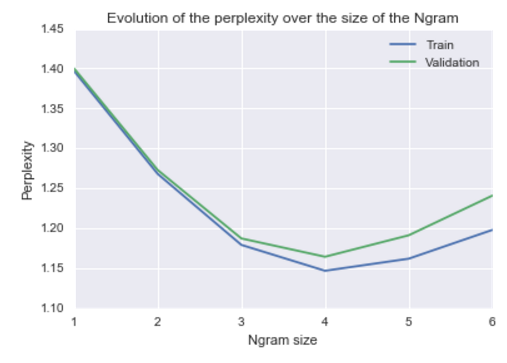
\includegraphics[width=0.45\textwidth]{count_graph.png}
    \caption{Perplexity evolution for the RNN}
\end{center}
\end{figure}

We observed an optimum of perplexity for the Ngram in both the validation and the train set. Then the steeper slope of the validation is due to overfitting. As a result, we sticked to this value for the model.\\

We implemented the greedy algorithm and the Viterbi one up to the trigram (so with a bigram as a context). Coding the Viterbi for larger Ngram size requires to cover more and more possibilities in our class $C$ (given the position of spaces in the sequence). 


\subsection{Neural Language Model}


\subsection{Recurrent Neural Networks}

For the three recurrent networks implemented, we have different parameters to take into account: 
\begin{itemize}
	\item batch size l
	\item length of sequences b
	\item embedding dimension emb
	\item number of epochs nEpochs
\end{itemize}

Choosing the right batch-size seems to be a tradeoff between performance and running time, a smaller one provides smaller perplexity but takes more time to run. The length of the sequence seems to provide good result when in the interval $[30,..,50]$ without significant peak so we kept values in this zone. We set the embedding dimension to 20 for the experiments with some prior explorations also.


\begin{figure}[H]
\begin{center}
    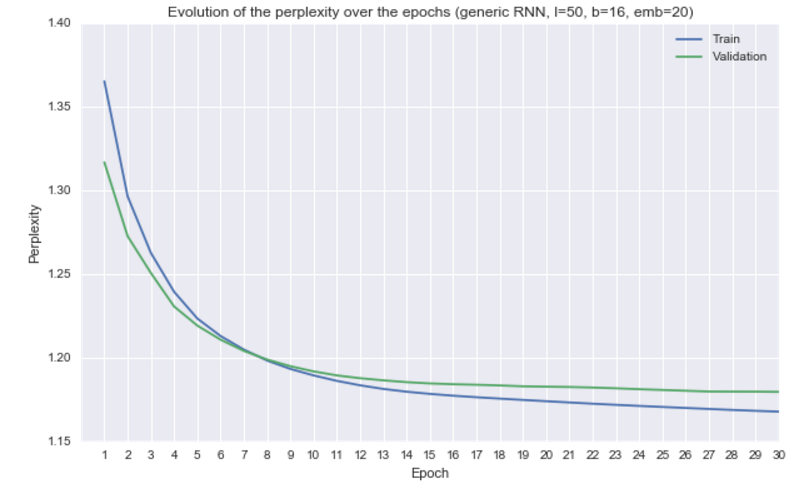
\includegraphics[width=0.45\textwidth]{perp_rnn.png}
    \caption{Perplexity evolution for the RNN}
\end{center}
\end{figure}

\begin{figure}[H]
\begin{center}
    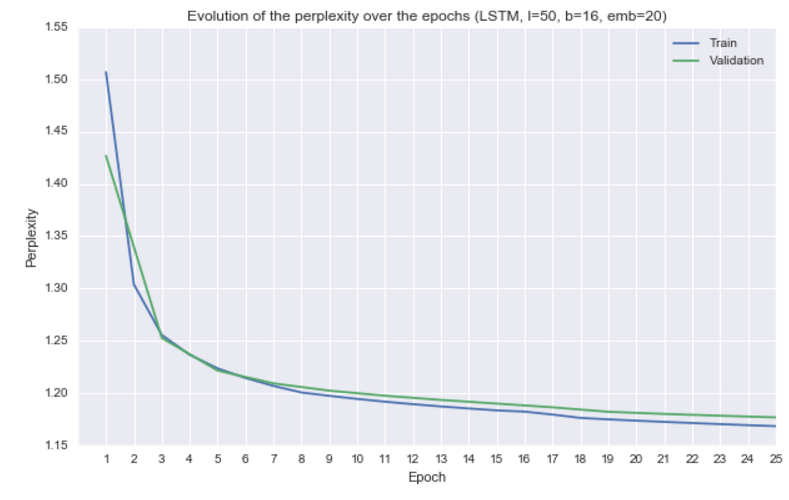
\includegraphics[width=0.45\textwidth]{perp_lstm.png}
    \caption{Perplexity evolution for the LSTM}
\end{center}
\end{figure}

\begin{figure}[H]
\begin{center}
    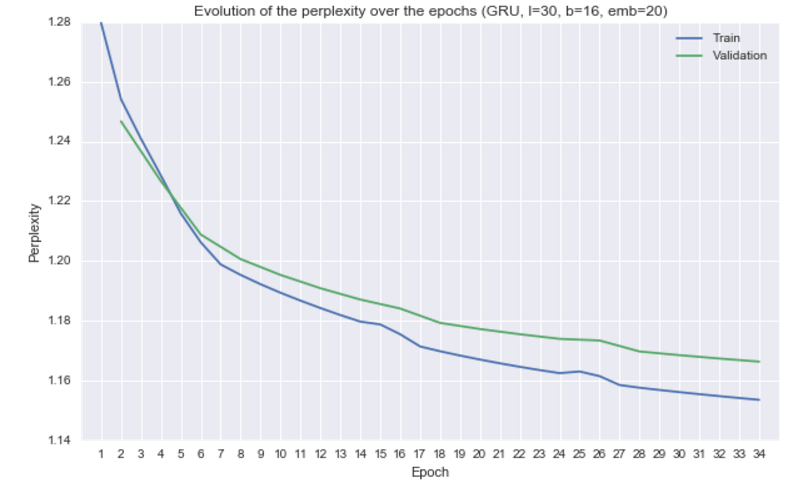
\includegraphics[width=0.45\textwidth]{perp_gru.png}
    \caption{Perplexity evolution for the GRU}
\end{center}
\end{figure}

The best results on the Kaggle were provided with the GRU after a large number of epochs (around 100).


\subsection{Model performance summary}

TABLE TO SUMMARIZE RESULT (perptrain, perpvalid, pred on kaggle)


\section{Conclusion}

End the write-up with a very short recap of the main experiments and the main results. Describe any challenges you may have faced, and what could have been improved in the model.

\bibliographystyle{apalike}
\bibliography{writeup}

\end{document}
